\chapter{Hernández Zavala Ana Sofía}

{\Large \texttt{¡Hola mundo!}}\vspace*{1em} \\ 
Soy Ana Sofía Hernández Zavala y nací el 29 de septiembre del 2003 en la ciudad de Tehuacán Puebla, actualmente acabo de cumplir los 18 años y soy hija única. Durante mis primeros años escolares estuve estudiando en este municipio, sin embargo decidí cursar el bachillerato en la ciudad de México. Desde pequeña se me ha facilitado el idioma inglés, aunque aún no me considero una experta hablandolo.\vspace*{0.5em}\\
\indent A los 14 años decidí que quería estudiar en una preparatoria de la ciudad de México, y gracias al apoyo de mis padres logré entrar en la Escuela Nacional Preparatoria plantel 5 José Vasconcelos de donde soy egresada. Durante ésta etapa me interesé por distintos ámbitos y áreas escolares; debo admitir que área 1 de ciencias e ingenierías no siempre fue lo que más me atraía, pues a lo largo de estos años adquirí gustos y disgustos por todas las áreas en general pues inclusive llegué a pensar en estudiar traducción, química o artes; pero área 1 predominó a la hora de elegir grupo en 6to grado.\vspace*{0.5em}\\
\indent A lo largo de estos 18 años he obtenido y eliminado ciertos pasatiempos pues anteriormente me gustaba dibujar, hacer manualidades o tocar intrumentos como el piano y el violin; pero ahora disfruto más nadar, ver una buena serie, hacer ejercicio, ver algún video interesante o documental en Deutsche Welle, escuchar música, de vez en cuando jugar ajedrez o platicar con mis amigos.\vspace*{0.5em}\\
\indent Decidí estudiar Ciencias de la Computación porque en la preparatoria elegí los Estudios Técnicos Especializados en Computación, también porque me gusta mucho la tecnología, las matemáticas, la programación, la inteligencia artificial y todo lo que se puede crear en base a ésta, más allá del desarrollo web o de aplicaciones y redes sociales, sino también los electrodomesticos, casas y ciudades inteligentes, avatares artificiales, e incluso la ciberseguridad.\\

\begin{figure}[h]
  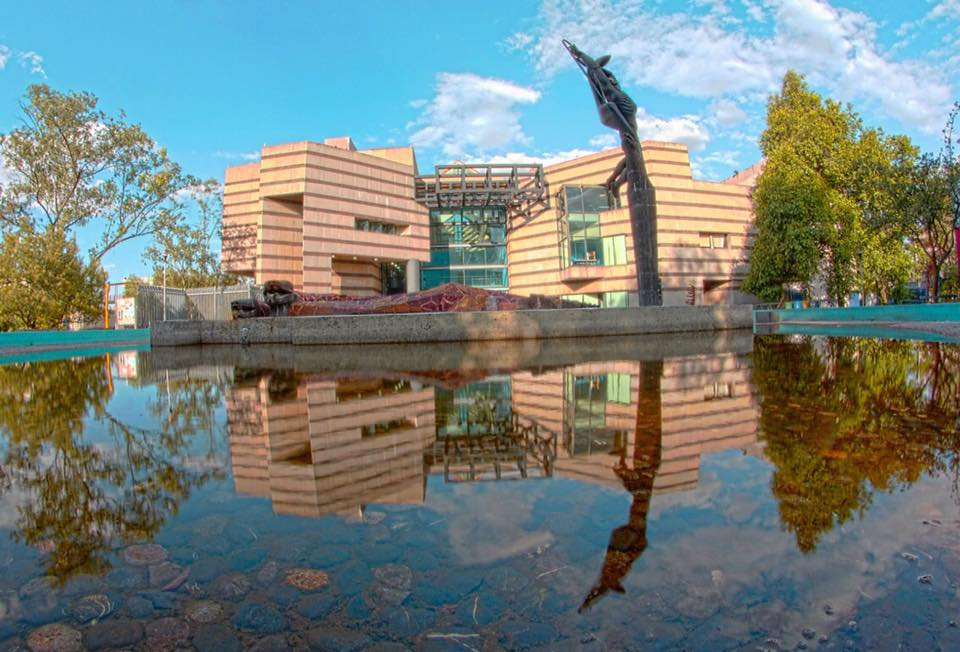
\includegraphics[scale=0.2]{319316717/Practica1.jpg}
  \centering
  \caption{Facultad de Ciencias UNAM, elegí esta imagen porque es la comunidad con la que me siento identificada}
\end {figure}

\begin{figure}[h]
  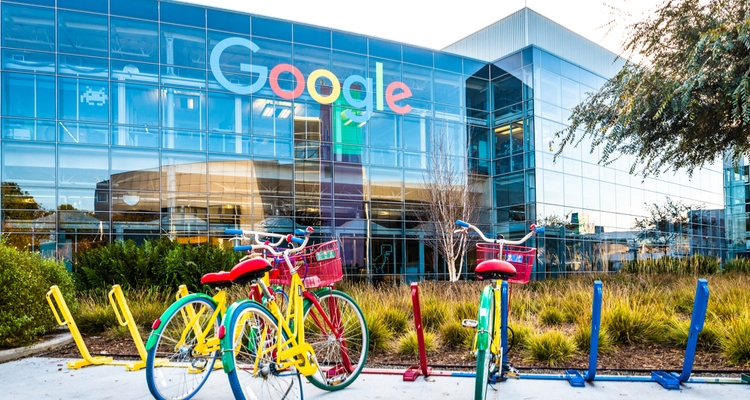
\includegraphics[scale=1.25]{319316717/Practica1a.jpg}
  \centering
  \caption{Edificios de Google, es importante para mi porque es donde en algún futuro quiero estar}
\end {figure}

\subsection*{\Large \centering \textsc{Teoréma del Binomio de Newton}}
\textbf{Teoréma del Binomio: }Sea $x, y$ números reales y $n$ un número natural; entonces se cumple:\\
\begin{aling*}
  (x+y)^n= \sum_{k=0}^{n}\binom{n}{k} x^{n-k}y^k\\
\end{aling*}
\begin{enumerate}
\item Base $n=0$\\
  \begin{equation}
  \begin{split}
    (x+y)^0 &= 1\\
    \sum_{k=0}^{0}\binom{0}{k} x^{0-k}y^k &= \binom{0}{0} x^{0-0}y^0\\
    &=1x^0y^0=1*1*1\\
    &=1\\
  \end{split}
  \end{equation}
\item Hipótesis inductiva\\ Supongase que $(x+y)^n= \sum_{k=0}^{n}\binom{n}{k} x^{n-k}y^k$ se cumple para una $n\in\mathds{N}$ fija.
\item Tesis inductiva\\ Si cumple para $n$, entonces debe de cumplir para $n+1$
  \begin{equation}
  \begin{split}
    (x+y)^{n+1}= \sum_{k=0}^{n+1}\binom{n+1}{k} x^{n+1-k}y^k \\
  \end{split}
  \end{equation}
\item Demostración\\
  \begin{equation}
  \begin{split}
    (x+y)^{n+1}&= (x+y)^n(x+y)^1\\
    &= \left( \sum_{k=0}^{n}\binom{n}{k} x^{n-k}y^k \right) \left(x+y \right) \\
    &= x \left( \sum_{k=0}^{n}\binom{n}{k} x^{n-k}y^k \right) + y \left(\sum_{k=0}^{n}\binom{n}{k} x^{n-k}y^k \right)\\
    &= \sum_{k=0}^{n}\binom{n}{k} x^{n-k}*x^1y^k + \sum_{k=0}^{n}\binom{n}{k} x^{n-k}y^1*y^k\\
    &= \sum_{k=0}^{n}\binom{n}{k} x^{n-k+1}y^k + \sum_{k=0}^{n}\binom{n}{k} x^{n-k}y^{1+k}\\
    &= \sum_{k=0}^{n}\binom{n}{k} x^{n-k+1}y^k + 0 + \sum_{k=0}^{n}\binom{n}{k} x^{n-k}y^{1+k}\\
    &= \sum_{k=0}^{n}\binom{n}{k} x^{n-k+1}y^k + \binom{n}{n+1} +\sum_{k=0}^{n}\binom{n}{k} x^{n-k}y^{1+k}\\
    &= \sum_{k=0}^{n+1}\binom{n}{k} x^{n-k+1}y^k + \sum_{k=1}^{n+1}\binom{n}{k-1} x^{n-(k-1)}y^{1+k-1}\\
    &= \sum_{k=0}^{n+1}\binom{n}{k} x^{n-k+1}y^k + \sum_{k=1}^{n+1}\binom{n}{k-1} x^{n-k+1}y^{k}+0\\
    &= \sum_{k=0}^{n+1}\binom{n}{k} x^{n-k+1}y^k + \sum_{k=1}^{n+1}\binom{n}{k-1} x^{n-k+1}y^{k}+ \binom{n}{-1} x^{n+1}y^{0}\\
    &= \sum_{k=0}^{n+1}\binom{n}{k} x^{n-k+1}y^k + \sum_{k=0}^{n+1}\binom{n}{k-1} x^{n-k+1}y^{k}\\
    &= \sum_{k=0}^{n+1} \left[ \binom{n}{k} x^{n-k+1}y^k + \binom{n}{k-1} x^{n-k+1}y^{k} \right]\\
    &= \sum_{k=0}^{n+1} x^{n-k+1}y^k \left[ \binom{n}{k}+\binom{n}{k-1} \right]\\
    &= \sum_{k=0}^{n+1} \binom{n+1}{k} x^{n-k+1}y^k\\
  \end{split}
  \end{equation}
\item Así queda demostrado
\end{enumerate}


